\documentclass[a4paper,12pt,pagesize,headsepline,bibliography=totoc,titlepage]{scrartcl}
\usepackage[utf8]{inputenc}
% \usepackage[T1]{fontenc}
\usepackage{mathptmx}
\usepackage[scaled=.90]{helvet}
\usepackage{courier}
\usepackage{amsmath,amsthm,amsfonts,graphicx,caption}
\usepackage{hyperref}
\usepackage{ae,aecompl}
\usepackage{todonotes}
\usepackage{subcaption}
\usepackage{listings}

\lstset {
	backgroundcolor=\color{white},
	breakatwhitespace=false,
	breaklines=true,
	numbers=left,
	frame=single,
	title=\lstname,
	basicstyle=\footnotesize
}

% \pagestyle{headings}
\headsep4mm % Abstand der Kopfzeile vom Text
% \typearea[current]{current}

\title{
	\includegraphics*[width=0.4\textwidth]{img/hpi_logo.png}\\
	\vspace{24pt}
	Sentence Boundary Detection
}
\subtitle{
	Seminar\\
	Practical Applications of Multimedia Retrieval\\
	Fall Semester 2015/2016
}
\author{
	Tanja Bergmann, Joseph Bethge, Stefan Bunk, Ricarda Schüler\\[12pt]
	Supervisor:\\
    Xiaoyin Che\\
	Dr. Haojin Yang\\
	Prof. Dr. Christoph Meinel
}
\date{\today}

\begin{document}
\maketitle
\tableofcontents
\newpage

\section{Introduction}
\label{sec:introduction}
Automatic Speech Recognition systems (ASR) have many practical applications nowadays, e.g., in dictation systems for medical documentation and journalism.
Another application comes from the rapidly increasing amount of videos available online on video platforms for entertainment and learning, such as Youtube\footnote{\url{youtube.com}}, Vimeo\footnote{\url{vimeo.com}}, Coursera\footnote{\url{coursera.org}} or OpenHPI\footnote{\url{open.hpi.com}}.
All of these benefit from automatically generated transcripts and subtitles.
However, the result of many ASR systems is an unformatted text without any punctuation marks, such as periods and commas.
These texts are hard to read and understand without manually inserting the missing punctuation marks.
However, this is a mundane, complicated task.
Therefore, an automatic solution for formatting the ASR output and inserting punctuation marks is necessary.
We call this \emph{sentence boundary detection} (SBD).

SBD is a mandatory preprocessing step for many further use cases.
For example, most machine translation outputs are trained on properly formatted text.
Having an ASR output without punctuation marks decreases the performance of machine translating systems.
Also, other natural language processing tasks, such as part-of-speech tagging or tokenization, work on sentence units.
Thus, the ASR output needs to be formatted before it can be further processed.

In this paper we want to address this problem by automatically creating punctuated text from unpunctuated text.
We use neural networks to process the unformatted transcripts.
The use of neural networks has led to large improvements in areas, such as image and video classification recently.

Our SBD system contains two models: one from the ASR text transcript (lexical model), and one from the raw audio data (acoustic model).
We train both models independently and retrieve their separate predictions.
Afterwards the results are combined in a fusion step.
The final output can replace the original output from ASR systems and improve readability and quality of transcripts.
Additionally, the punctuation marks often represent suitable boundaries for subtitles, enhancing their overall quality.

The rest of the paper is structured as follows:
Related work is summarized in Section~\ref{sec:related_work}.
Section~\ref{sec:training_data} describes the datasets we use for training and evaluation.
The data preprocessing, training, and evaluation of our lexical and our acoustic model can be seen in Section~\ref{sec:lexical_model} and Section~\ref{sec:acoustic_model} respectively.
Details of the fusion step are explained in Section~\ref{sec:fusion}.
We show our demo application in Section~\ref{sec:demo} and conclude our work in Section~\ref{sec:future}.

\section{Related Work}
\label{sec:related_work}
As punctuation prediction is a mandatory preprocessing step for further working with automated speech recognition output, a lot of research has been done in this field.
Some approaches focus only on the lexical part~\cite{Gravano2009, Lu2010, Ueffing2013, Cho2012, Zhang2013}.
Gravano et al.~\cite{Gravano2009} used a text-based n-gram language model to detect punctuation (comma, period, question mark).
Dynamic conditional random fields are used by Lu and Ng~\cite{Lu2010} and Ueffing et al.~\cite{Ueffing2013}.
Ueffing et al. evaluate their method with different features, like language model scores, parse trees, dynamic sentence length and token n-grams.
The usefulness of the individual features highly depends on the nature of the text, which is processed.
For example, if the text is well structured, the parse tree features improve the result.
Similar to our approach, Cho et al.~\cite{Cho2012} use a sliding window over the input data to predict different punctuations.
Zhang et al.~\cite{Zhang2013} predict punctuations of an input stream.
For each processed word in the input stream, syntactic features are used to predict the punctuation symbol after that word.
The used features include, e.g., part-of-speech tags, tree-based features (the parse tree is build step by step) or bag of words.

Most of the researchers combine prosodic features, such as pitch, pauses, duration, and lexical features, such as words, n-grams, part-of-speech tags~\cite{Mark1999, Christensen2001, Liu2005, Matusov2007, Wang2012}.
Mark and Mark~\cite{Mark1999} predict punctuation on the basis of prosodic features in a first step using a Hidden Markov Model.
In a second step they use a language model to adapt the predicted punctuation from the first step.
Christensen et al.~\cite{Christensen2001} focus on multi-layer perceptron methods to combine prosodic and lexical features, whereas Liu et al.~\cite{Liu2005} use conditional random fields.
Matusov et al.~\cite{Matusov2007} optimize their approach to the needs of machine translation.
They combine a language model and prosodic features in a log-linear model and add a phrase coverage feature, which is motivated by phrase-based machine translation systems.
A comparison of different machine learning models to combine prosodic and lexical feature for the prediction of punctuation was done by Wang et al.~\cite{Wang2012}.
The dynamic conditional random fields achieve the best result on a broadcast news copora (F1-Measure of 42.8\%).

In this paper we present a new approach: predicting punctuations using deep learning.
To the best of our knowledge, such an approach was never tried before.
We learn two individual models, one based on lexical features and the other one based on prosodic features.
In the end, the predictions of both models are fused.

% \subsection{Distributed Representations}
% word2vec
% Würde ich kurz related work zu schreiben, wenn wir es erwähnen
% \subsection{Caffe}


\section{Training Data}
\label{sec:training_data}
% how did we prepare our data


\section{Lexical Model}
\label{sec:lexical_model}
In this chapter we describe how we predict the position of periods, commas and question marks in unpunctuated text using lexical features.
The used data is described in Section \ref{sec:training_data}.

The system is based on the deep learning framework \emph{caffe}.
Therefore the processing pipeline is the following:

\begin{itemize}
\item preprocess the data, so that it can be used as input for caffe
\item train the network with the preprocessed data
\item retrieve predictions for new data
\item transform the output into a valuable result
\end{itemize}

\subsection{Data Preprocessing}

For processing the data, we need to extract features which caffe can handle.
Since you can not use a whole text as input, we decided to use a sliding window to generate training and testing instances.
A sliding window is in our case, that we split a sentence like \emph{The sun is shining and we go outside} into the following pieces (assuming a window size of 5):
\begin{itemize}
\item the sun is shining and
\item sun is shining and we
\item is shining and we go
\item shining and we go outside
\end{itemize}

We call these pieces instances and the window size directly defines how many words are in each instance.
The label of each instance is then whether there is a punctuation (and which one) at a defined position.
We call this position punctuation position.
In the above example every instance would have a label of \emph{None} with a punctuation position of 2, since there is no punctuation.

After we split up the sentences into instances we convert each word into a distributed word representation.
We use the distributed word representation described earlier: \emph{word2vec}. \todo{Insert word2vec link. Describe Word2Vec in related work?}
The final model we used for our distributed word representation was trained on google news entries \todo{Link and/or paper}.
Since not every word exists in the trained model, we use the word vector representing \emph{this} for unknown words.
We think that most of the unknown words are proper names, which can easily be replaced with \emph{this} without changing the meaning and structure of the whole sentence.

We also figured out that the trained model only contains the number \emph{1} and a few more of the most common numbers instead of all numbers. \todo{Check whether only 1 is in the word vector or whether numbers like 12 and 5 are also contained}
That is why we replace any number with \emph{1}.

The representation for each word in an instance is inserted into one row of the feature matrix, e.g. for a sliding window size of 5 you get the matrix of 5x300 for each instance.

Besides the distributed word representation we also examined Part of Speech (POS) tags as features.
We used the nltk POS tagger to identify the POS tags with the whole text as input.
The tagger distinguishes between 35 different POS tags.
These are too specific for our purpose, so we reduced them into 14 different categories.
For example we combined CD and LS to a more generic category \emph{numeral}.
The nltk tagger predicts more than one tag per word, so one word can have multiple tags (even after reducing the tag categories).
To allow the existence of multiple tags in our feature matrix, we used the following representation:
We create one flag per POS category which has the value 1 if the word belongs to this category and 0 otherwise.

There are two possibilities to include them.
On the one hand it is possible to append all flags at the end to word vector representations.
On the other hand an extra channel with the flags can be used.

For all further testing, wherever we used the POS-features, we decided to append the flags to the vector representation of the words.
Therefore the resulting feature matrix for a sliding window size of 5 with POS tags is 5x314.

% Data preparation
% Windowing
% Config.ini File

% Google Vector

\subsection{Neural Network Layout}

We use a neural network layout with three main \texttt{innerproduct} layers with sizes 2048, 4096, and 2048.
After each of these layers we added a \texttt{ReLU} and a \texttt{dropout} layer on top of each \texttt{innerproduct} layer.
The ratio for all \texttt{dropout} layers is $0.5$.
Accuracy and loss of the network are computed after the final predictions of our fourth \texttt{innerproduct} layer wih size 3 or 4 depending on the number of punctuation symbols.

\subsection{Evaluation}
Formeln für Precision, Recall, Harmonic Mean
Evaluation, wikipidia usage?, results with wikipedia test set

Evaluation of results:
\begin{itemize}
\item F-measure for each class is calculated.
\item Harmonic mean for all F-measures is total score (higher is better).
\end{itemize}

\begin{figure}[ht]
    \centering
    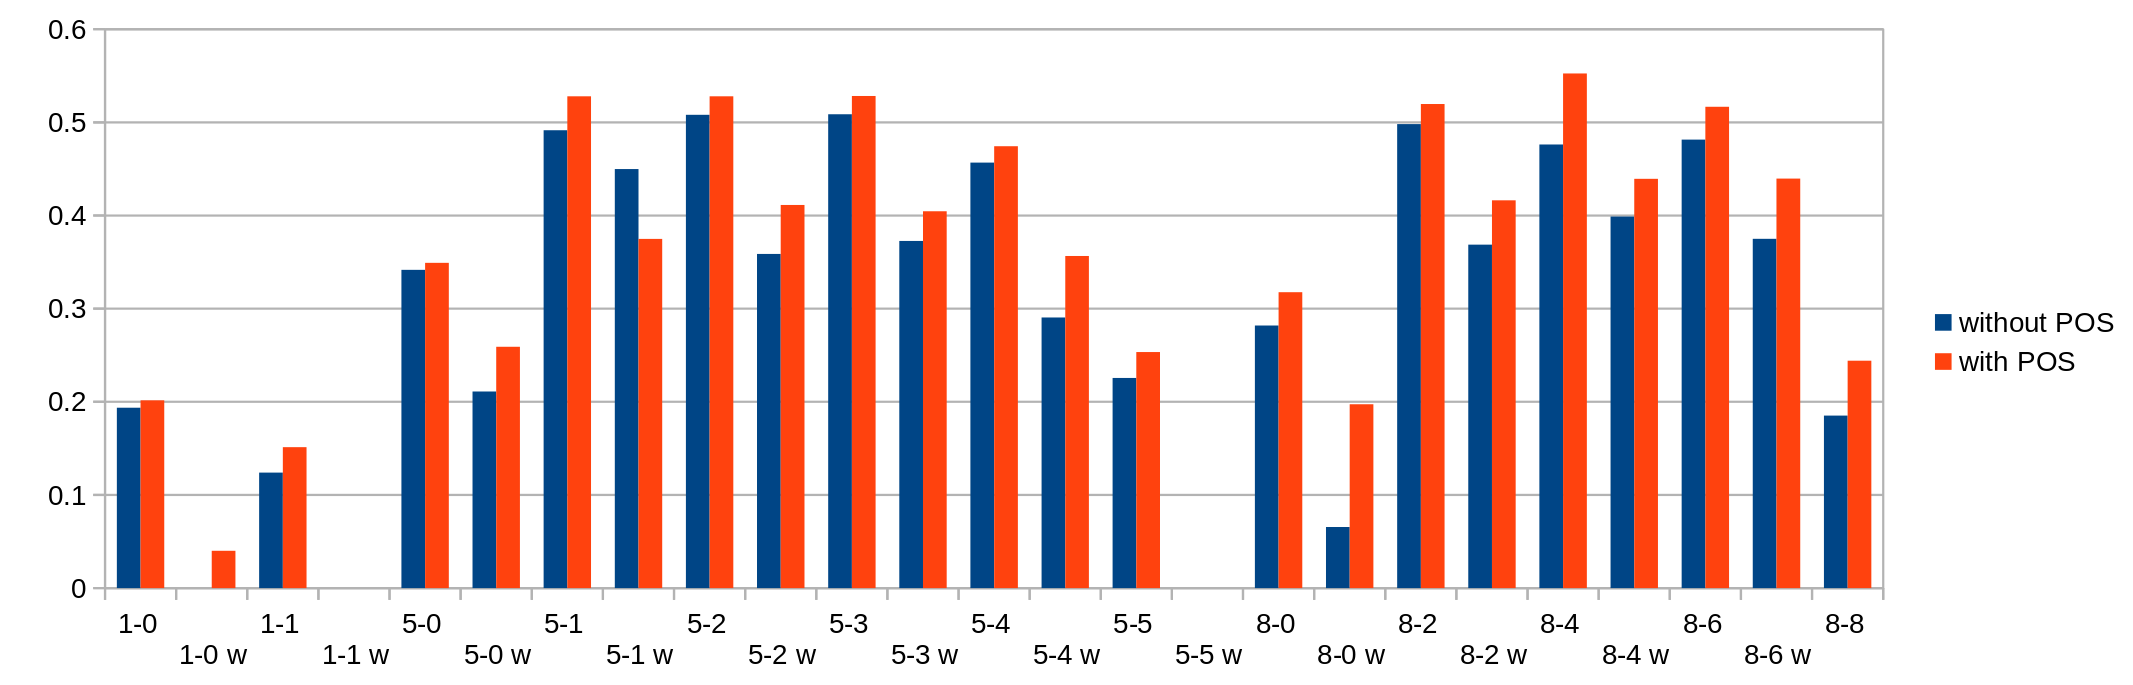
\includegraphics[width=\textwidth]{img/window_eval.png}
    \caption{Harmonic mean between all f1 scores for all classes. \emph{2/5} means window size of five and punctuation position two. If \emph{wi} is in the label, it uses wikipedia training data.}
    \label{window_eval}
\end{figure}

\begin{figure}[ht]
    \centering
    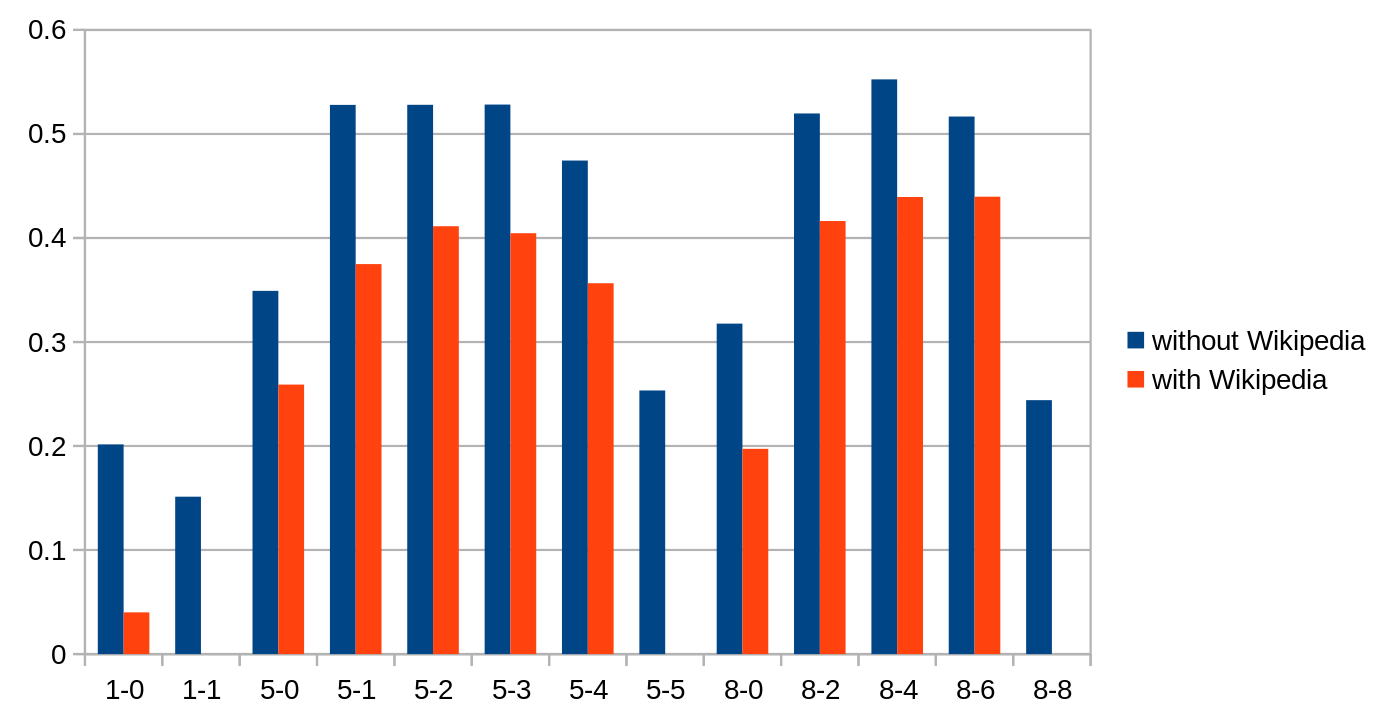
\includegraphics[width=\textwidth]{img/window_wiki_eval.png}
    \caption{}
    \label{window_wiki_eval}
\end{figure}

\begin{figure}[ht]
    \centering
    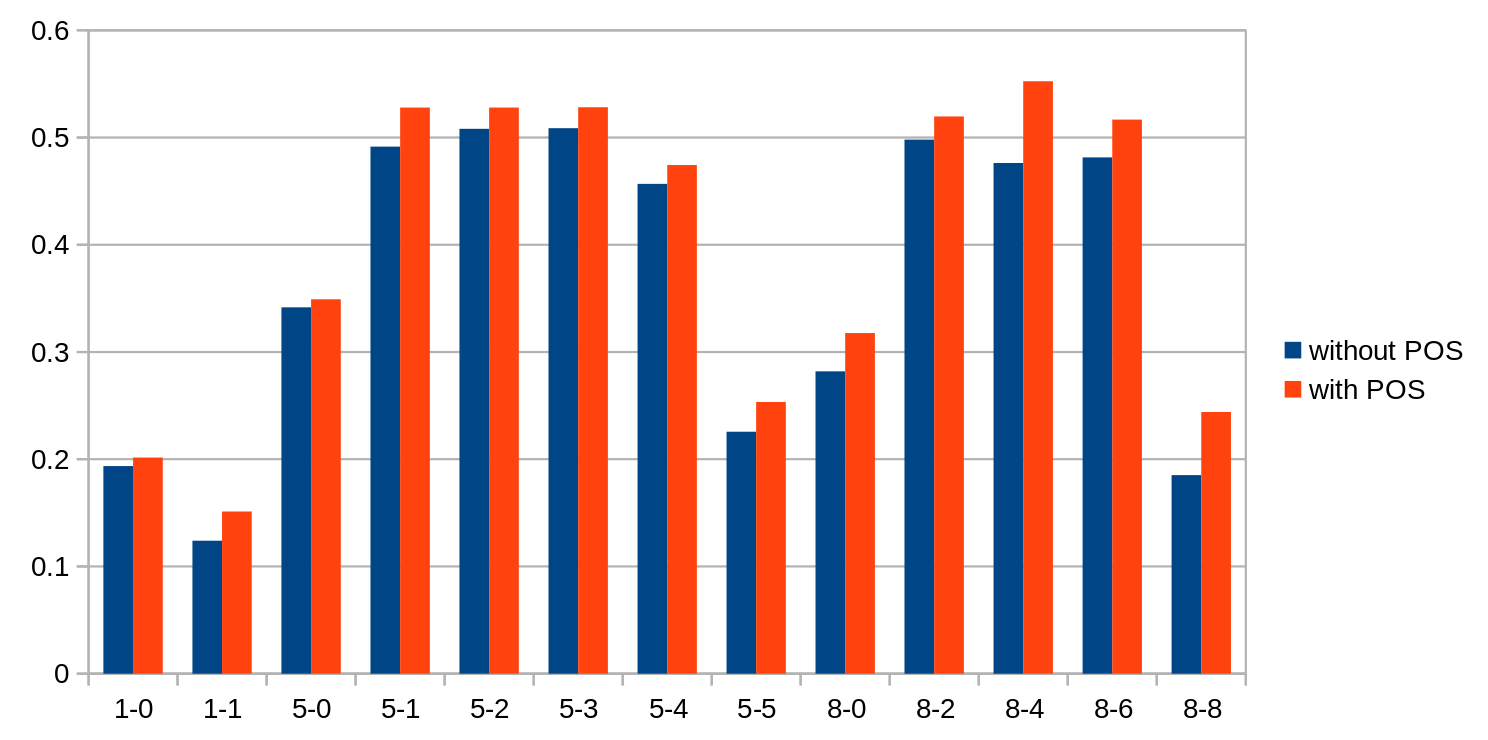
\includegraphics[width=\textwidth]{img/window_pos_eval.png}
    \caption{}
    \label{window_pos_eval}
\end{figure}

Comparison between experiments with and without POS tagging (other than that, they have the same configurations):
\begin{itemize}
\item With POS tagging: 0.305
\item Without POS tagging: 0.275
\end{itemize}

Comparison between experiments with and without wikipedia data (other than that, they have the same configurations):
\begin{itemize}
\item Without wikipedia: 0.385
\item With wikipedia data: 0.252
\end{itemize}


\section{Acoustic Model}
\label{sec:acoustic_model}
\begin{figure}[ht]
    \centering
    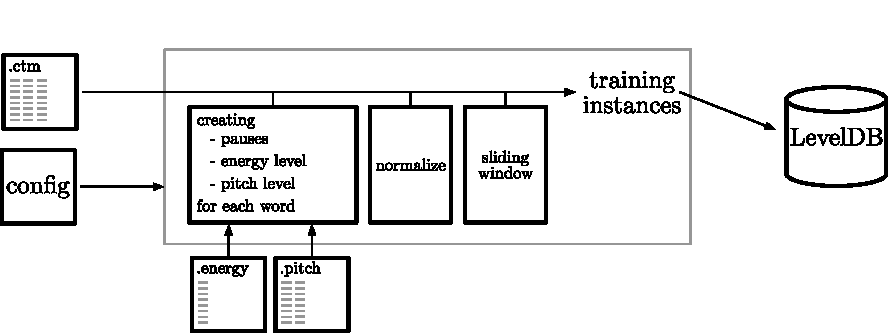
\includegraphics[width=\textwidth]{img/overview_accoustic.pdf}
    \caption{}
    \label{fig:overview_accoustic}
\end{figure}

\begin{figure}[ht]
    \centering
    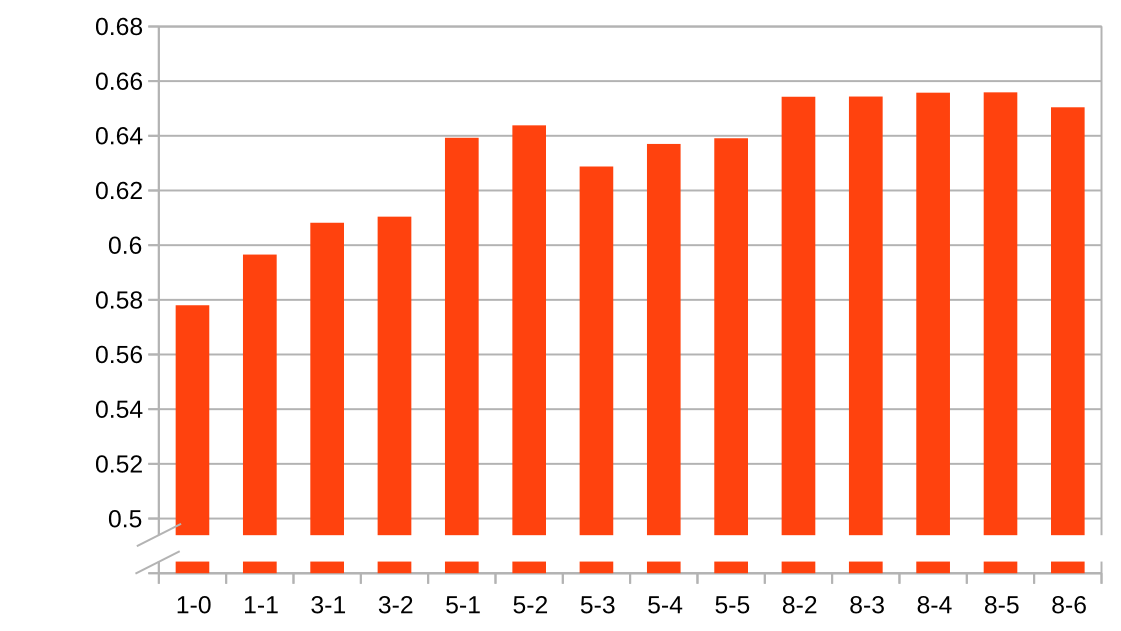
\includegraphics[width=\textwidth]{img/audio_parameter_eval.png}
    \caption{}
    \label{audio_eval}
\end{figure}

\section{Fusion}
\label{sec:fusion}
The individual predictions from the acoustic and the lexical model need to be combined to obtain a final, overall prediction.
Therefore, we fuse the predictions of the two models.
We implemented two different fusion approaches: 
The first approach is called \emph{Threshold Fusion}, the second \emph{Balance Fusion}.
The two fusion approaches and the evaluation will be presented in the remainder of this section.

\subsection{Threshold Fusion}
The main idea of the threshold fusion is the following: If the probability for the class \textsc{Period} from the acoustic model is over a certain threshold and the probability for the class \textsc{None} from the lexical model is below a certain threshold, we want to predict a period or a comma.
If the condition is satisfied, the probability of the class \textsc{Period} from the acoustic model is added to the probabilities of the classes \textsc{Period} and \textsc{Comma} from the lexical model.
The idea of the threshold fusion is shown in the Figure~\ref{fig:fusion_1}.
\begin{figure}[ht]
    \centering
    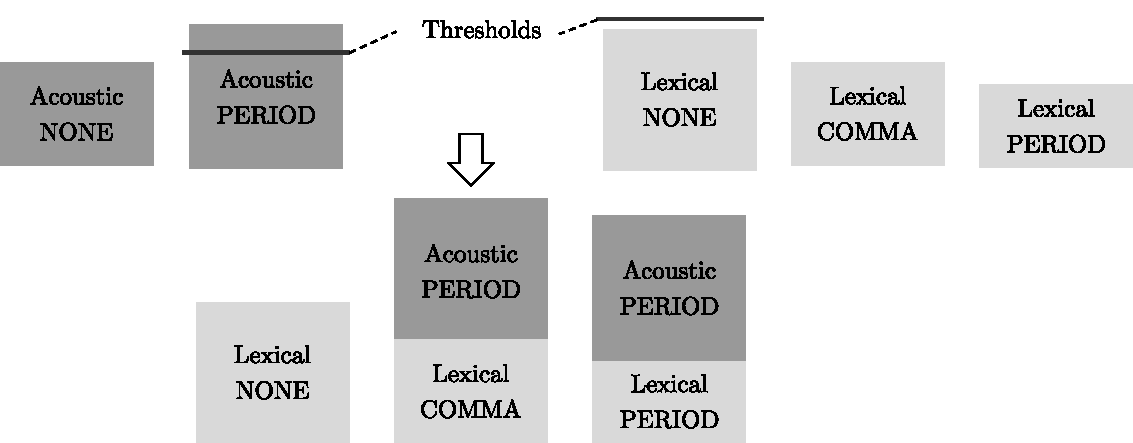
\includegraphics[width=0.7\textwidth]{img/fusion_1.pdf}
    \caption{Threshold Fusion: The probability of the class \textsc{Period} from the acoustic model is added to the probabilities of the classes \textsc{Period} and \textsc{Comma} from the lexical model, if the probability for the class \textsc{Period} from the acoustic model is over a certain threshold and the probability for the class \textsc{None} from the lexical model is below a certain threshold.}
    \label{fig:fusion_1}
\end{figure}
If the condition holds not, just the predictions of the lexical model are taken as final the predictions.
Thus, the threshold fusion trusts the lexical model more than the acoustic model.
The acoustic model is only taken into account, if the acoustic model is quite certain, that there should be a period, and the lexical model is not certain enough, that there should be no punctuation at all.
In the end, the class with the highest probability is chosen.
For the example in Figure~\ref{fig:fusion_1}, we would predict a comma. 

\subsection{Balance Fusion}
The balance fusion sums up weighted probabilities of both models.
Figure~\ref{fig:fusion_2} shows an example.
\begin{figure}[ht]
    \centering
    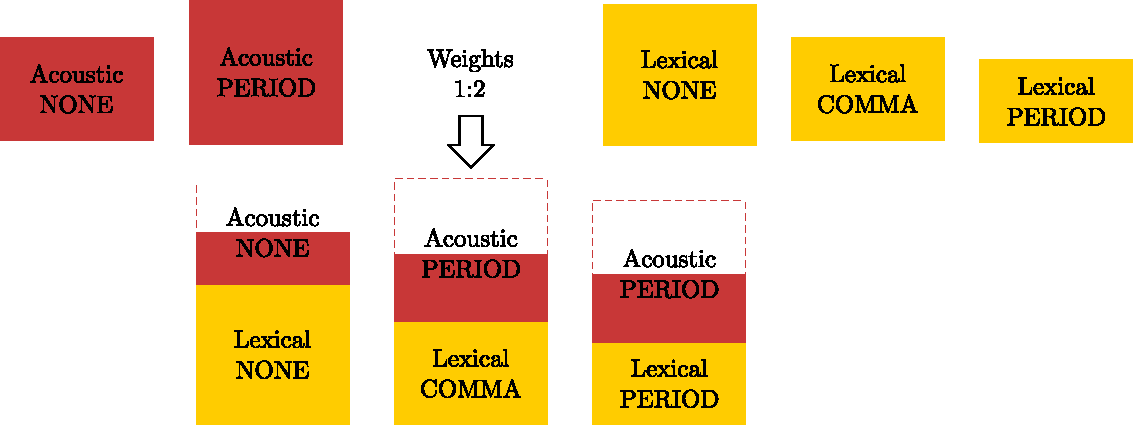
\includegraphics[width=0.7\textwidth]{img/fusion_2.pdf}
    \caption{Balance Fusion: Sum up the weighted probabilities of both models.}
    \label{fig:fusion_2}
\end{figure}
Using weights we can regulate, which model we trust more.
In the example shown in Figure~\ref{fig:fusion_2}, the lexical model is more important than the acoustic model. 
In the end, the class with the overall highest probability is chosen again.
So in the example, this would be the class \textsc{None}.

\subsection{Evaluation}


\section{Demo Tool}
\label{sec:demo}
We use a demo application, accessible with a web browser, to present the working prototype.
It can be used to find sentence boundaries in unpunctuated text.
The general web page shows two main tabs, one labeled \emph{Lexical} and one \emph{Lexical + Audio}.
A user can click these, to switch between using only the lexical model or the fusion of both the lexical and the acoustic model.

There are two ways to feed input to our model for the \emph{Lexical} SBD (see Figure~\ref{fig:demo_l}).
\begin{figure}[ht]
    \centering
    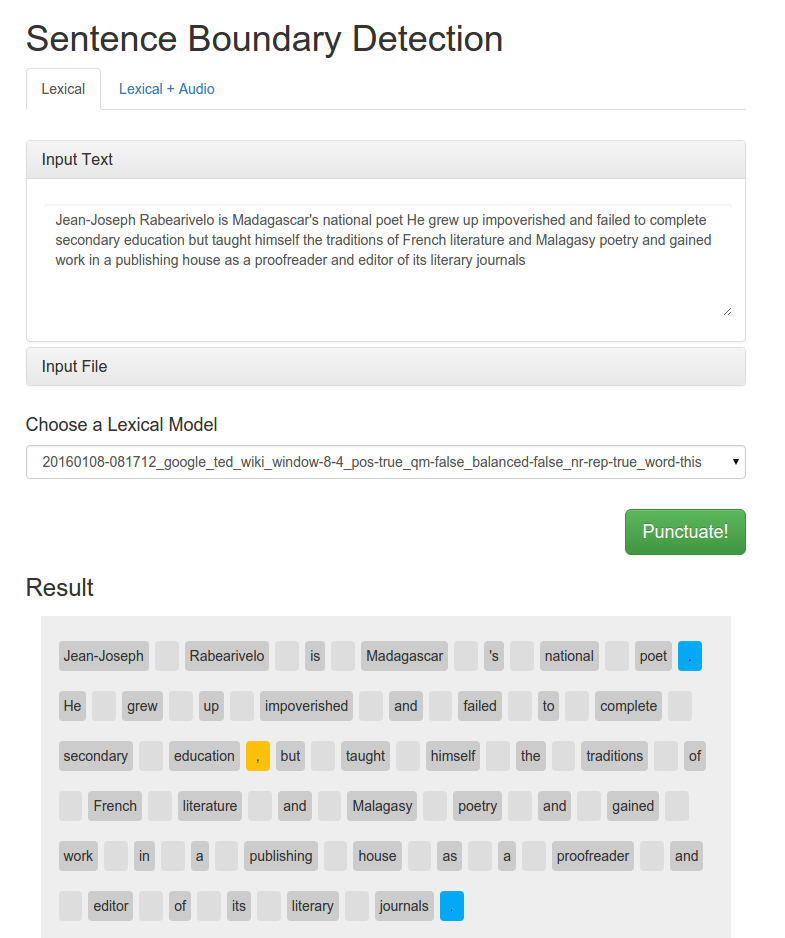
\includegraphics[width=0.5\textwidth]{img/demo_l.png}
    \caption{The demo application for lexical model. The results are presented below the options for input and model selection.}
    \label{fig:demo_l}
\end{figure}
The user can enter a text input field to manually enter or paste any text they wish.
Another possibility is to choose from a set of existing text files.
A dropdown selection allows the user to choose the pretrained models, if multiple models are available in the system.
If the model is changed, it is automatically loaded in the background.
Once the user clicks the \emph{Punctuate!} button, the text, which was entered, or selected as a file, is passed to our lexical model.
While the server processes the request, a small loading icon is shown inside the button.
After the predictions are returned from the server, the result is shown beneath.
The input text and positions where no punctuation was predicted are shown as tokens with a light grey background.
Any commas or periods inserted, are shown in distinct colors.
If a model, which uses POS tags, is selected a user can hover their mouse over a token to see its POS category.
For further use the entire result is selectable and can be copied.

For the \emph{Lexical + Audio} SBD the possibilities for entering input are more limited (see Figure~\ref{fig:demo_la}).
\begin{figure}[ht]
    \centering
    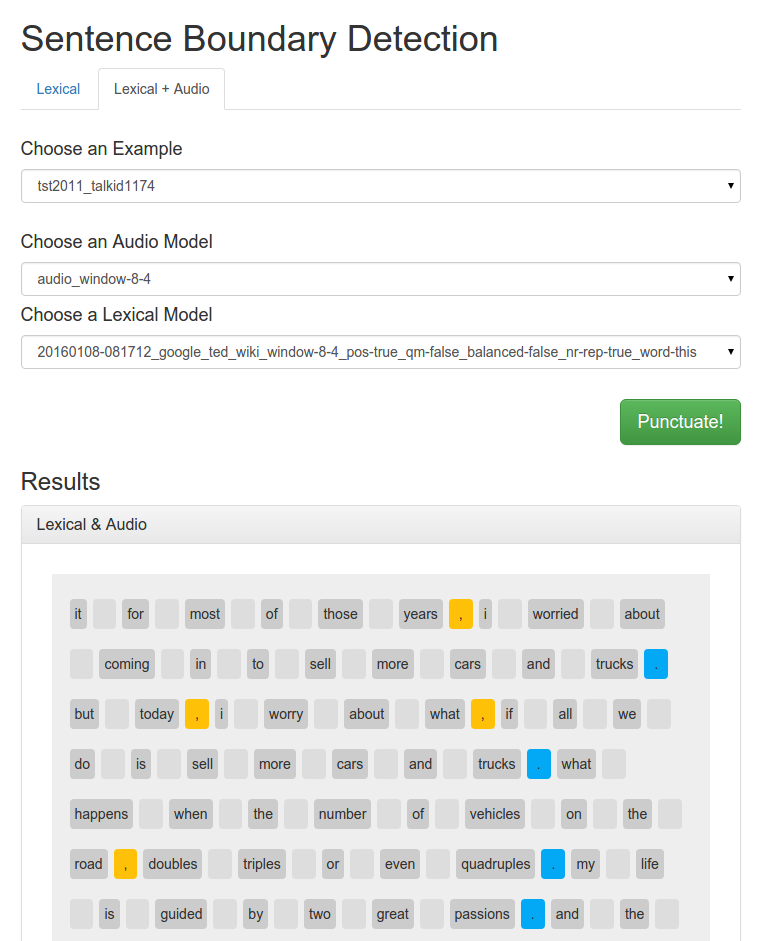
\includegraphics[width=0.5\textwidth]{img/demo_l_a.png}
    \caption{The demo application for fusion of both models. The results of the individual models and the fusion are presented below the options for input and model selection. Only one result section is in the screenshot, the other sections are out of the region of the screenshot.}
    \label{fig:demo_la}
\end{figure}
Since we need an audio recording, we only offer examples existing in the system.
At the moment the system contains samples, which were used in the testing phase, but not for training.
The selection of the user is therefore limited by a dropdown menu of all available choices.
However, the choice of both the acoustic and the lexical model is independently available to a user.
These can also be selected in a dropdown menu.
The functionality of the \emph{Punctuate!} button is unchanged.
It triggers the processing and shows a loading indicator until the result returns.
The result area however is changed, and contains three subareas, which each contain a different result.
Two of them contain the raw results of the acoustic model and the lexical model.
The third shows the result after the fusion.
Therefore, it is easy to compare the results of each individual model, and the result after the fusion.


\section{Future Work}
\label{sec:future}
We presented an approach to automatically detect sentence boundaries, and predict the correct punctuation marks in unpunctuated ASR output.
Two different models were trained independently, one using lexical input and the other using acoustic input.
The results of both models were merged with a late fusion.
Evaluation has shown, that one has to be careful with the training data, which should stem only from actually spoken text.
Just adding more written text data did not improve the performance.
On the other hand, part of speech tags as additional features consistently increase the performance of the sentence boundary detection.

There are many possibilities for improvement on the presented approach.
Since we did not explore the large variety of different neural network layouts, further exploration in this area is likely to improve on the results.
Especially in the case of more training data, a deeper network architecture can provide better results.
Also, using Long Short Term Memory (LSTM) neural networks appears promising, as they can process a stream of data while keeping time information.
This maps easily to the stream of word tokens in a text.

In the fusion step we decided for a late fusion approach, which combines only the predictions.
However, another way to explore, is an earlier fusion, where both models and the fusion itself are trained together.
Instead of fusing the predictions, the actual features can be fused.
As for data preparation, a different representation of features in the lexical model can be examined, such as a second or third data channel or a combination similar to the fusion of the acoustic and lexical model.

Another improvement could be achieved with a better post processing of the results.
For example, one punctuation symbol right after another is unlikely to be correct.

\bibliographystyle{plain}
\bibliography{bibliography.bib}

\newpage
\appendix
\section{Appendix}
We appended the following files for reference:
\begin{itemize}
    \item lexical-solver.prototxt, the configuration of the solver (lexical model)
    \item lexical-net.prototxt, our net configuration (lexical model)
    \item acoustic-solver.prototxt, the configuration of the solver (acoustic model)
    \item acoustic-net.prototxt, our net configuration (acoustic model)
\end{itemize}

\subsection{lexical-solver.prototxt}
\lstinputlisting[caption={lexical-solver.prototxt}, label={lst:lexical-solver.prototxt}]{../net/solver.prototxt}
\newpage

\subsection{lexical-net.prototxt}
\lstinputlisting[caption={lexical-net.prototxt}, label={lst:lexical-net.prototxt}]{../net/net.prototxt}
\newpage

\subsection{acoustic-solver.prototxt}
\lstinputlisting[caption={acoustic-solver.prototxt}, label={lst:acoustic-solver.prototxt}]{../net-audio/solver.prototxt}
\newpage

\subsection{acoustic-net.prototxt}
\lstinputlisting[caption={acoustic-net.prototxt}, label={lst:acoustic-net.prototxt}]{../net-audio/net.prototxt}

%\newpage %for more appended files

\end{document}
